\pagebreak
\subsection{System Administration}
\label{sec:system-admin}

The previous sections of our evaluation primarily focused on performance using our custom deployment scripts. However, in order to complete our evaluation of the Ceph file system, we have additionally evaluated Ceph's official deployment tools on our test cluster. To that end, we will detail our findings in this section.

Ceph's setup differs significantly to that of a traditional \ac{HPC} file system. Specifically, the containerization of Ceph services results in particularly relaxed requirements for the host operating system. In addition to the most common \ac{HPC} operating systems on the TOP500 list\footnote{\url{https://top500.org/statistics/sublist/}. Accessed 26.02.2026.}, such as Red-Hat derivatives (e.g., Rocky Linux) and Ubuntu, system requirements are relaxed such that any modern Linux distribution with the base requirements is adequate for a functional Ceph installation\footnote{\url{https://docs.ceph.com/en/reef/cephadm/install/\#requirements}. Accessed 26.02.2026.}---the internal container image is based on CentOS Stream 9\footnote{Checked using the \texttt{/etc/os-release} file within the Ceph containers deployed with cephadm.}.

\subsubsection{Initial Setup}

The following steps were taken in order to build a functional cluster on our virtual machine setup based on the Ceph instructions\footnote{\url{https://docs.ceph.com/en/reef/cephadm/install/}. Accessed 26.02.2026.}:

\begin{sloppypar}
\begin{itemize}
    \item Cephadm was installed using the curl-based method
    \item \texttt{cephadm bootstrap} was used to bootstrap the cluster on the first node \texttt{cvm1}
    \item The created \ac{SSH} public key was copied to the root user's authorized keys of the other nodes in the cluster
    \item \texttt{ceph orch host add cvmX --labels \_admin} was used from \texttt{cvm1} (with X being 2--8), in order to add \texttt{cvm2}--\texttt{cvm8} to the cluster
    \item \acp{OSD} were added based on available hard disks using the command \texttt{ceph orch apply osd -{}-all-available-devices}
\end{itemize}
\end{sloppypar}

\subsubsection{Accessing the Ceph Dashboard}

After initial bootstrapping, we were presented with credentials, which we were able to use to access the Ceph dashboard.

\lstinputlisting[
    caption={
        [Ceph Bootstrap Output]
        Output at the end of the Ceph bootstrapping phase, showing the credentials for accessing the Ceph dashboard.
    },
    label={lst:ceph-bootstrap},
    frame=single,
    breaklines=true
]{assets/ceph/bootstrap_output.txt}

\pagebreak
\begin{figure}[H]
    \centering
    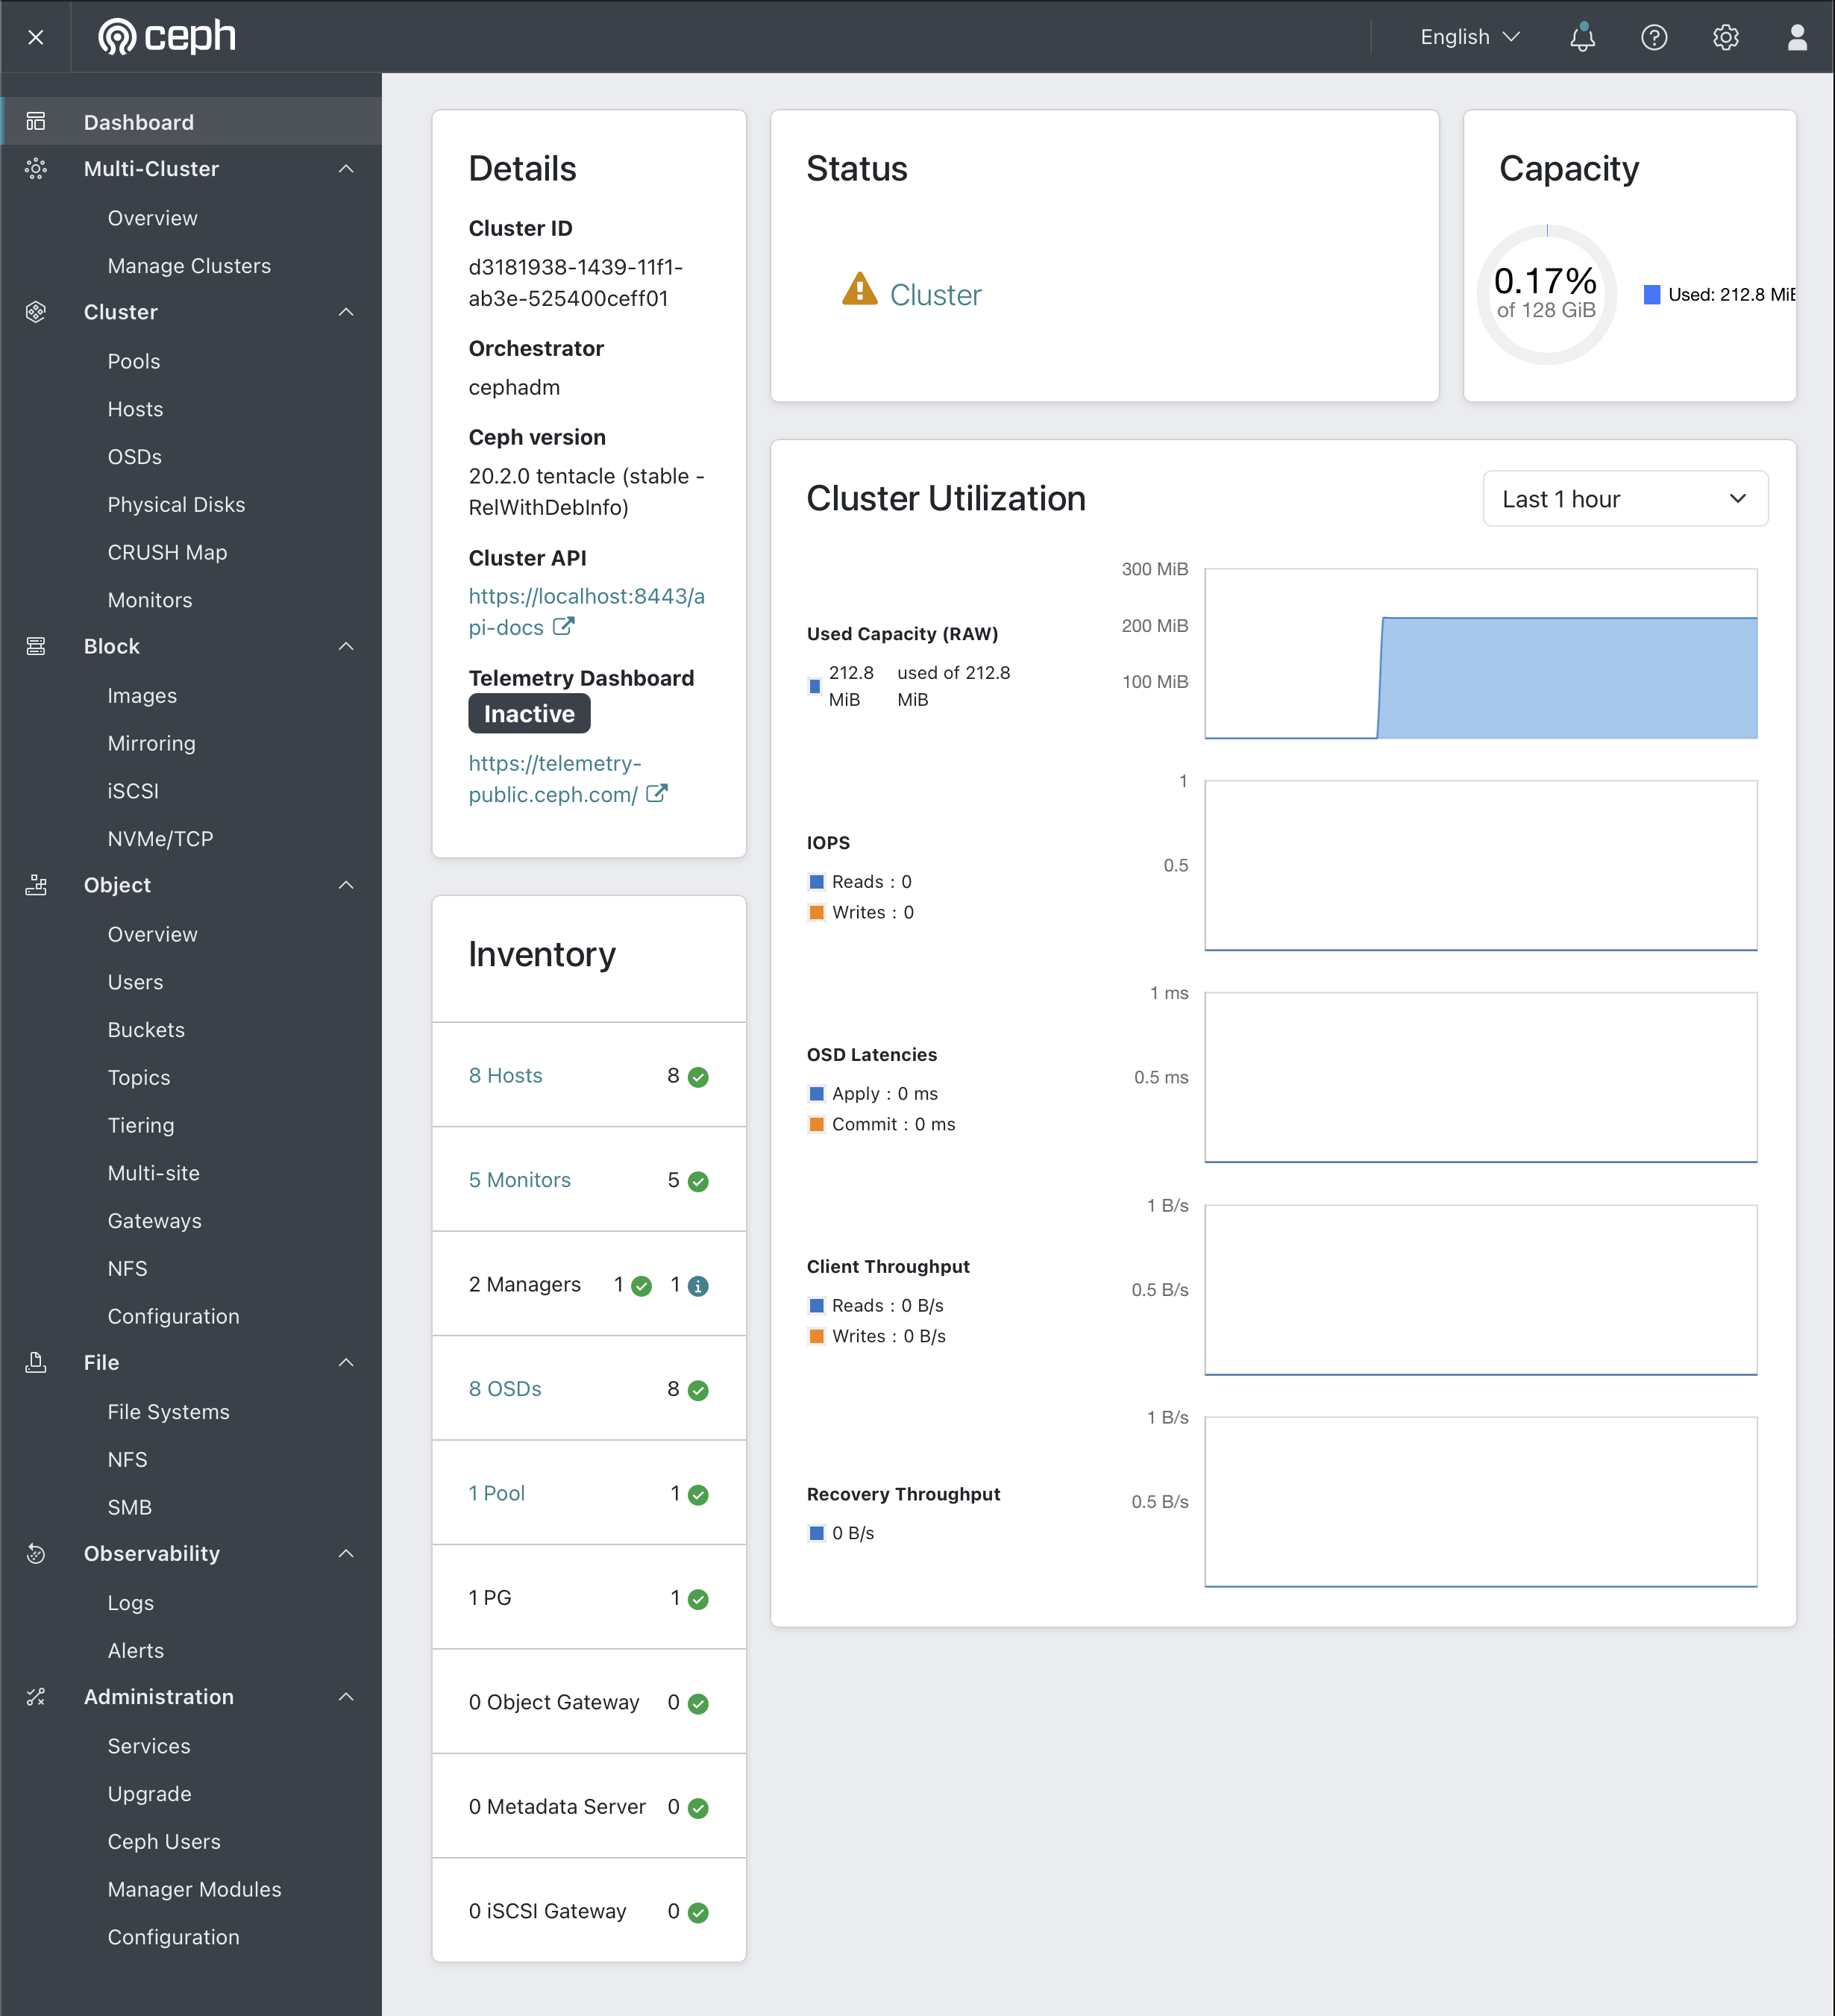
\includegraphics[width=0.99\textwidth]{assets/ceph/ceph-dashboard.png}
    \caption{The Ceph Dashboard}
    \label{fig:ceph-dashboard}
\end{figure}

The Ceph dashboard provides a web-based interface for monitoring and managing the cluster without the need for experience with the Ceph \ac{CLI}. A screenshot of the dashboard of the deployed cluster is shown in~\cref{fig:ceph-dashboard}. We were able to perform common monitoring tasks successfully using the dashboard, such as viewing free space, monitoring disk activity, and checking other health metrics of the cluster. In addition to these basic features, the dashboard is also capable of performing more advanced tasks\footnote{\url{https://docs.ceph.com/en/quincy/mgr/dashboard}. Accessed 26.02.2026.}, and is being actively developed. The monitoring stack is based on Prometheus, which allows for a high degree of customizability and external access, in addition to integration with other tools such as Grafana.

\pagebreak
\subsubsection{Potential System Administration Issues}
\label{sec:system-admin-issues}

We have identified a number of minor issues and bugs in Ceph's system administration aspect.

\subsubsection*{User Interface Inconsistency}

Adding \acp{OSD} via \texttt{ceph orch} worked as expected. However, the user interface refresh delay resulted in some confusion, as the status of the disks was not immediately updated. We added the disks to the cluster with the orchestrator as shown in~\cref{lst:osd-add-initial}.

\lstinputlisting[
    caption={Adding \acsp{OSD} via \texttt{ceph orch}},
    label={lst:osd-add-initial},
    frame=single,
    breaklines=true
]{assets/ceph/osd_add_initial.txt}

However, the outputs from various Ceph daemons took several minutes to synchronize with each other, which caused some confusion when determining the cluster's actual state. \Cref{lst:osd-sync-issue} demonstrates the inconsistent reporting of various Ceph commands.

\lstinputlisting[
    caption={
        [\acs{OSD} Synchronization Delay]
        \acs{OSD} synchronization delay after adding disks. The device list shows available disks, but the \acsp{OSD} are reported as down. Outputs are truncated.
    },
    label={lst:osd-sync-issue},
    frame=single,
    breaklines=true
]{assets/ceph/osd_sync_issue.txt}

\begin{sloppypar}
In order to synchronize the system, restarting the manager daemons was required, for which we used \texttt{ceph orch restart mgr}. After this step, the status commands showed the expected output, as shown in~\cref{lst:osd-after-restart}.
\end{sloppypar}

\lstinputlisting[
    caption={
        [\acs{OSD} Status After Manager Daemon Restart]
        \acs{OSD} status after a restart of the manager daemons.
    },
    label={lst:osd-after-restart},
    frame=single,
    breaklines=true
]{assets/ceph/osd_after_restart.txt}

\subsubsection*{Adding \ac{OSD} Disks}

When attempting to check the system for new \acp{OSD}, the reject reason does not clearly state that the reason specific \acp{OSD} may be rejected are due to the fact that these disks already host a Ceph \ac{OSD}, as the error message states only that a file system is on the disk, not necessarily one used by Ceph, as shown in~\cref{lst:osd-reject-reasons}.

\lstinputlisting[
    caption={
        [\acs{OSD} Rejection Reasons for Existing Ceph Disks]
        Rejection reasons for existing Ceph disks when attempting to add \acsp{OSD}.
    },
    label={lst:osd-reject-reasons},
    frame=single,
    breaklines=true
]{assets/ceph/osd_reject_reasons.txt}

\subsubsection*{Reinstallation Quirks}

In the Ceph documentation, it is mentioned that a cluster can be purged with cephadm\footnote{\url{https://docs.ceph.com/en/quincy/cephadm/operations/}. Accessed 26.02.2026.}. However, we found that this did not cleanly purge all traces of the cluster, leaving behind residual daemons which complicated future reinstallations of the cluster due to clashes with existing daemons left behind on the cluster, including after a reboot.

\lstinputlisting[
    caption={
        [Residual Node-Exporter Daemons]
        Residual node-exporter container remaining after the cluster purge command was run.
    },
    label={lst:residual-node-exporter},
    frame=single,
    breaklines=true
]{assets/ceph/residual_node_exporter.txt}

\lstinputlisting[
    caption={
        [Residual Ceph Daemons]
        Residual Ceph daemons from multiple clusters remaining after the cluster purge command was run.
    },
    label={lst:residual-daemons},
    frame=single,
    breaklines=true
]{assets/ceph/residual_daemons.txt}

When we manually removed the containers after running the Ceph purge and restarted the virtual machines, we were able to successfully initialize a new cluster from scratch.

% Modern Ceph deployments rely on the use of the \texttt{cephadm} tool. Because this tool uses standard \ac{SSH} connections to connect to and set up hosts, as well as Podman as a container runtime for running Ceph daemons

% In this section, we primarily discuss the system administration of the Ceph file system, from cluster setup to common maintenance tasks.

% Setup of the cluster was rather straightforward, and documentation on the bootstrapping phase was clear and concise. The cephadm tool was downloaded on the host node, and bootstrapping was performed successfully